\begin{frame}[t]
\frametitle{The Execution Model}
  \begin{itemize}
    \item Several objects live on a single {\em PE} 
%     \begin{itemize}
%       \item We will come back what we mean by a PE
      \begin{itemize}
        \item For now, think of it as a core (or just ``processor'')
      \end{itemize}
%     \end{itemize}
  \pause
  \item As a result, 
    \begin{itemize}
      \item Method invocations directed at objects on that processor will have to be stored in a pool,
      \pause
      \item And a user-level scheduler will select one invocation from the queue and runs it to completion
      \item A PE is the entity that has one scheduler instance
           associated with it
    \end{itemize}
  \end{itemize}
  \begin{center} 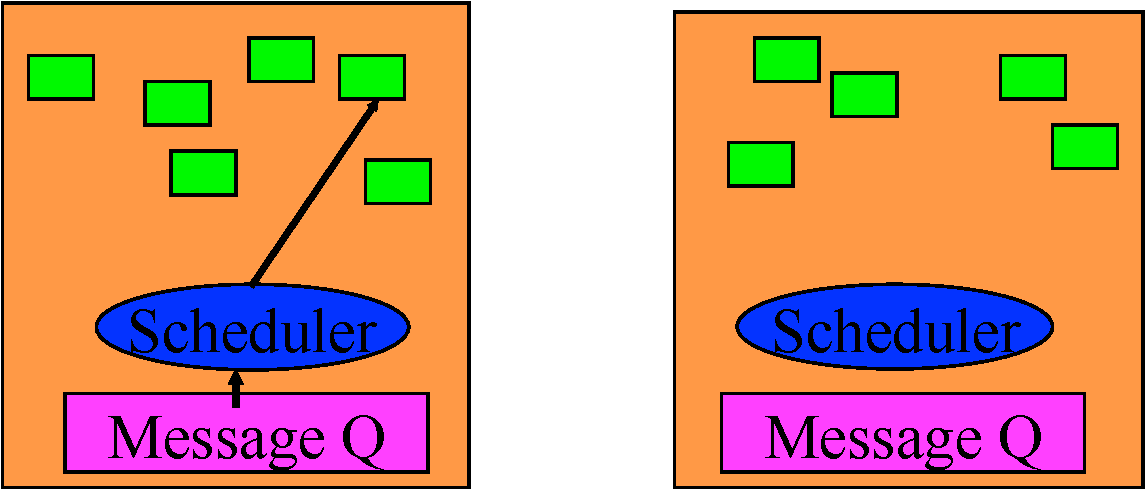
\includegraphics[width=0.7\textwidth]{figures/scheduler} \end{center}
\end{frame}

\begin{frame}[t]
\frametitle{Message-driven Execution}
  \begin{itemize}
    \item Execution is trigggered by availability of a ``message'' (a method invocation)
    \pause
    \item When an entry method executes, 
    \begin{itemize}
      \item it may generate messages for other objects
      \item the RTS deposits them in the message Q on the target processor
    \end{itemize}
  \end{itemize}
  \begin{center} 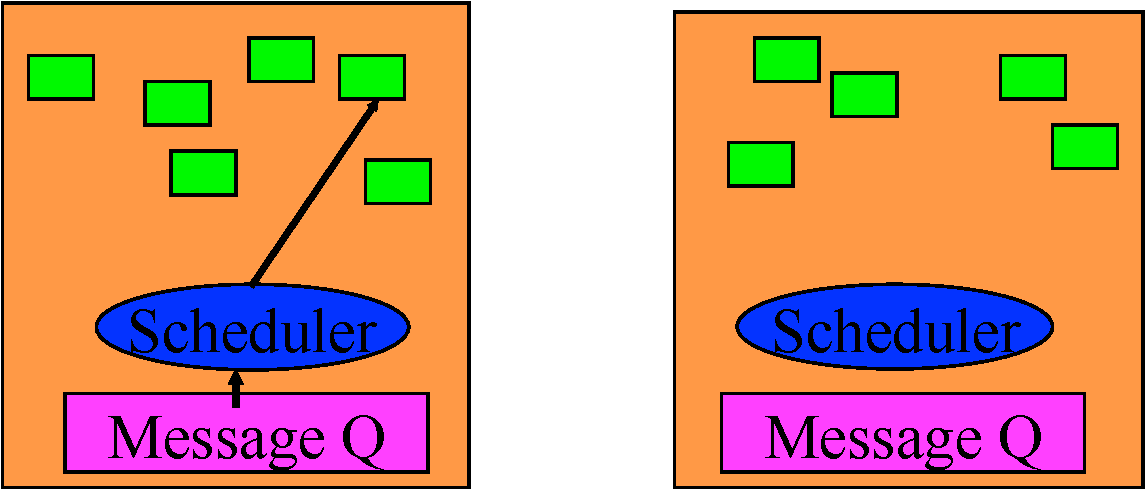
\includegraphics[width=0.7\textwidth]{figures/scheduler} \end{center}
\end{frame}

\begin{frame}[t]
\frametitle{Utility for Multi-cores, Many-cores, Accelerators}
  \begin{itemize}
    \item Objects connote and promote locality
    \item Message-driven execution is
    \begin{itemize}
      \item A strong principle of prediction for data and code use
      \item Much stronger than principle of locality
      \begin{itemize}
        \item Can be used to scale memory wall
        \item Prefetching of needed data, e.g, into scratch pad memories
      \end{itemize}
    \end{itemize}
  \end{itemize}
  \begin{center} 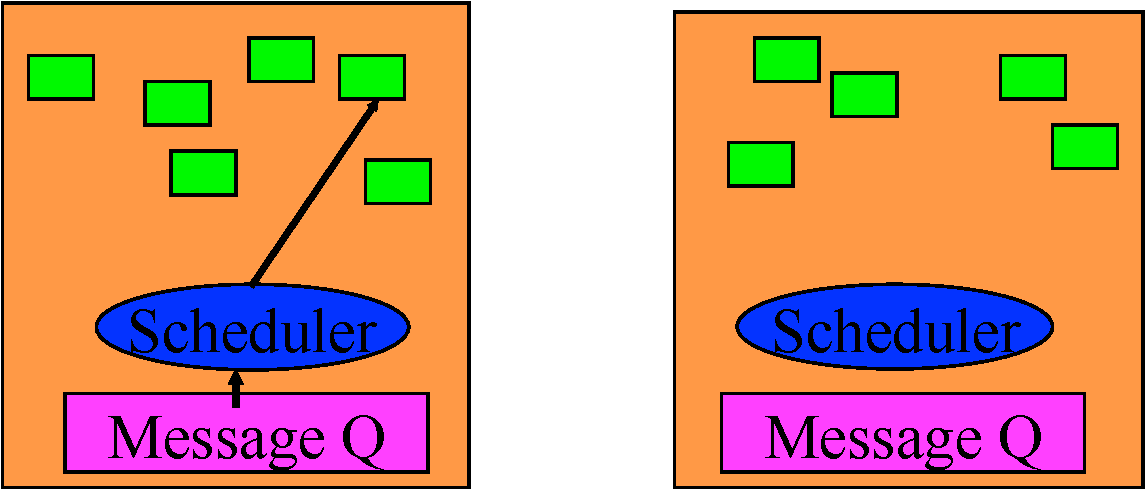
\includegraphics[width=0.7\textwidth]{figures/scheduler} \end{center}
\end{frame}




